% Mensuration: DSE revision worksheet.
% Compile this file for the student copy.
% Compile worksheet-answers.tex for the copy with full marking-scheme solutions.
% Every twin's arithmetic is checked by ../tools/check_twins.py.
\documentclass[11pt,addpoints]{exam}
% Shared preamble for the Mensuration revision handouts.
\usepackage[a4paper,margin=18mm,top=16mm,bottom=18mm]{geometry}
\usepackage{amsmath,amssymb}
\usepackage{enumitem}
\usepackage{booktabs,array,tabularx}
\usepackage{multicol}
\usepackage[dvipsnames]{xcolor}
\usepackage[most]{tcolorbox}
\usepackage{lastpage}

\definecolor{wyblue}{HTML}{004898}
\definecolor{wyred}{HTML}{D7000F}
\definecolor{wygrey}{HTML}{6D6E71}

% Function names in upright type, as in HKEAA papers.
\def\f{\mathrm{f}}  \def\g{\mathrm{g}}  \def\h{\mathrm{h}}
\def\p{\mathrm{p}}  \def\q{\mathrm{q}}  \def\F{\mathrm{F}}

\newcommand{\mk}[1]{\hfill\textnormal{(#1)}}
\newcommand{\src}[1]{{\small\color{wygrey}[#1]}}

\tcbset{
  box/.style={enhanced, sharp corners, boxrule=0.6pt, colframe=wyblue, colback=white,
              coltitle=white, colbacktitle=wyblue, fonttitle=\bfseries, left=6pt, right=6pt,
              top=4pt, bottom=4pt, before skip=6pt, after skip=6pt},
  trap/.style={enhanced, sharp corners, boxrule=0pt, borderline west={2pt}{0pt}{wyred},
              colback=white, left=8pt, right=4pt, top=2pt, bottom=2pt, before skip=4pt, after skip=4pt},
}
\newtcolorbox{toolbox}[1]{box, title={#1}}
\newtcolorbox{trapbox}{trap}

\setlength{\parindent}{0pt}
\setlength{\parskip}{3pt}

\usepackage{tikz}
\ifdefined\ANSWERS \printanswers \fi
\renewcommand{\solutiontitle}{\noindent\textbf{\color{wyblue}Solution}\par\noindent}
\unframedsolutions
\SolutionEmphasis{\color{black}}
\renewcommand{\choicelabel}{\thechoice.}
\pointsinrightmargin
\pointformat{}
\renewcommand{\questionlabel}{\textbf{\thequestiontitle}}
% MC options start on their own line.
\let\oldoneparchoices\oneparchoices
\renewcommand{\oneparchoices}{\par\smallskip\oldoneparchoices}
\newcommand{\qmarks}[1]{\hfill(#1 marks)}
% Tighter spacing so each section fits on one page.
\renewcommand{\questionshook}{\setlength{\itemsep}{3pt}\setlength{\topsep}{2pt}}
\renewcommand{\partshook}{\setlength{\itemsep}{0pt}\setlength{\topsep}{1pt}}
\renewcommand{\subpartshook}{\setlength{\itemsep}{0pt}\setlength{\topsep}{0pt}}
\newcommand{\cm}[1]{\text{ cm}^{#1}}

\pagestyle{headandfoot}
\firstpageheader{}{}{}
\runningheader{\small F6 Mathematics}{\small Mensuration: DSE Revision Worksheet\ifdefined\ANSWERS\ (Answers)\fi}{}
\runningheadrule
\footer{}{\small Page \thepage\ of \numpages}{}

\begin{document}

\hfill\textbf{F6 Mathematics}\par
\vspace{2pt}{\color{wyred}\rule{\linewidth}{1pt}}\par
{\LARGE\textbf{Mensuration: DSE Revision Worksheet}}\ifdefined\ANSWERS\ {\Large\color{wyred}(Answers)}\fi\par
\vspace{4pt}
\ifdefined\ANSWERS
Each question is a \emph{twin} of a real DSE question: same shape, new numbers. The bracket after each question names the paper it copies. Marks are shown in the DSE marking-scheme style: M = method mark, A = answer mark, f.t. = follow-through.
\else
Name: \rule{6cm}{0.4pt}\quad Class: \rule{1.5cm}{0.4pt}\quad No.: \rule{1.2cm}{0.4pt}

Every question below is a \emph{twin} of a real DSE question: same shape, new numbers.
\textbf{In class:} A1--A4 (5 minutes), then B2 under exam conditions (7 minutes).
\textbf{Homework:} everything else. Write Section B on foolscap, as in the DSE answer book. Target times: about \textbf{75 seconds} per MC and \textbf{1 minute per mark} for Section B.
\fi

\section*{Section A \quad Paper 2 style (multiple choice)}

\begin{questions}
\titledquestion{A1}
The perimeter and the area of a sector are $k\cm{}$ and $2k\cm2$ respectively. If the radius of the sector is $12\cm{}$, then the arc length of the sector is
\begin{oneparchoices}
  \choice $8\cm{}$. \CorrectChoice $12\cm{}$. \choice $16\cm{}$. \choice $24\cm{}$.
\end{oneparchoices}
\begin{solution}
Let $\ell\cm{}$ be the arc length. Area $= \frac12 r\ell$: $\;2k = \frac12(12)\ell = 6\ell$, so $k = 3\ell$.\\
Perimeter $= 2r + \ell$: $\;24 + \ell = 3\ell$, so $\ell = 12$. \quad \textbf{Answer: B} \src{twin of 2026 P2 Q16}\\
\emph{Key move:} area $= \frac12 r\ell$ links the area and the arc without the angle. \emph{Trap:} the perimeter includes the two radii.
\end{solution}

\titledquestion{A2}
\begin{minipage}[t]{0.7\linewidth}
In the figure, $OAB$ and $OCD$ are sectors with centre $O$, where $OA = 12\cm{}$ and $OC = 18\cm{}$. The area of the shaded region $ABDC$ is $30\pi\cm2$. Which of the following is/are true?
\begin{enumerate}[label=\Roman*., leftmargin=2.2em, nosep]
\item The angle of the sector $OAB$ is $60^\circ$.
\item The area of the sector $OAB$ is $24\pi\cm2$.
\item The perimeter of the sector $OCD$ is $6\pi\cm{}$.
\end{enumerate}
\begin{oneparchoices}
  \choice I only \choice II only \CorrectChoice I and II only \choice I, II and III
\end{oneparchoices}
\end{minipage}\hfill
\begin{minipage}[t]{0.26\linewidth}
\vspace{-6pt}\centering
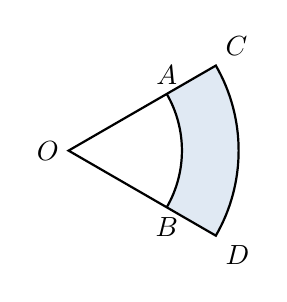
\begin{tikzpicture}[scale=0.12]
\fill[wyblue!12] (-30:12) arc (-30:30:12) -- (30:18) arc (30:-30:18) -- cycle;
\draw[thick] (0,0) -- (-30:18) arc (-30:30:18) -- cycle;
\draw[thick] (-30:12) arc (-30:30:12);
\node[left] at (0,0) {$O$};
\node[above] at (30:12) {$A$}; \node[below] at (-30:12) {$B$};
\node[above right] at (30:18) {$C$}; \node[below right] at (-30:18) {$D$};
\end{tikzpicture}
\end{minipage}
\begin{solution}
Let $\theta^\circ$ be the angle. $\frac{\theta}{360}\,\pi(18^2 - 12^2) = 30\pi$, so $\frac{\theta}{360}(180) = 30$ and $\theta = 60$. \;I is true.\\
Area of sector $OAB = \frac{60}{360}\pi(12^2) = 24\pi\cm2$. \;II is true.\\
Perimeter of sector $OCD = 2(18) + \frac{60}{360}(2\pi)(18) = (36 + 6\pi)\cm{}$. \;III is false (it gives the arc only). \quad \textbf{Answer: C} \src{twin of 2016 P2 Q19}
\end{solution}

\titledquestion{A3}
The diameter of a circle is $26\cm{}$. The circle is divided into a major segment and a minor segment by a chord of length $24\cm{}$. Find the area of the major segment correct to the nearest $\text{cm}^2$.
\begin{oneparchoices}
  \choice $139\cm2$ \choice $272\cm2$ \choice $332\cm2$ \CorrectChoice $392\cm2$
\end{oneparchoices}
\begin{solution}
Radius $13\cm{}$. The distance from the centre to the chord is $\sqrt{13^2 - 12^2} = 5\cm{}$, and the angle at the centre is $2\sin^{-1}\frac{12}{13} \approx 134.76^\circ$.\\
Minor segment $= \pi(13^2)\frac{134.76^\circ}{360^\circ} - \frac12(24)(5) \approx 198.74 - 60 = 138.74\cm2$.\\
Major segment $= \pi(13^2) - 138.74 \approx 392\cm2$. \quad \textbf{Answer: D} \src{twin of 2022 P2 Q16}\\
\emph{Traps:} A is the minor segment; C is the major \emph{sector} without the triangle.
\end{solution}

\titledquestion{A4}
The base of a solid right pyramid is a square of side $16\cm{}$. If the height of the pyramid is $15\cm{}$, then the total surface area of the pyramid is
\begin{oneparchoices}
  \choice $736\cm2$. \CorrectChoice $800\cm2$. \choice $1\,056\cm2$. \choice $1\,344\cm2$.
\end{oneparchoices}
\begin{solution}
The slant height of each triangular face is $\sqrt{15^2 + 8^2} = 17\cm{}$.\\
Total surface area $= 16^2 + 4\times\frac12(16)(17) = 256 + 544 = 800\cm2$. \quad \textbf{Answer: B} \src{twin of 2019 P2 Q15}\\
\emph{Trap:} using the height $15$ instead of the slant height gives A.
\end{solution}

\titledquestion{A5}
The base of a right pyramid is a rectangle. The length and the breadth of the base are $18\cm{}$ and $12\cm{}$ respectively. The height of the pyramid is $15\cm{}$. The pyramid is divided into a pyramid $X$ and a frustum $Y$ by a plane parallel to its base. If the breadth of the base of $X$ is $8\cm{}$, then the volume of $Y$ is
\begin{oneparchoices}
  \choice $320\cm3$. \choice $360\cm3$. \choice $600\cm3$. \CorrectChoice $760\cm3$.
\end{oneparchoices}
\begin{solution}
Volume of the whole pyramid $= \frac13(18)(12)(15) = 1080\cm3$. $X$ and the whole pyramid are similar with $k = \frac{8}{12} = \frac23$.\\
Volume of $Y = 1080\left[1 - \left(\frac23\right)^3\right] = 1080 \times \frac{19}{27} = 760\cm3$. \quad \textbf{Answer: D} \src{twin of 2026 P2 Q17}\\
\emph{Traps:} A is $X$, not $Y$; C uses $k^2$ instead of $k^3$.
\end{solution}

\titledquestion{A6}
If the volume of a right circular cylinder of base radius $3a\cm{}$ and height $4b\cm{}$ is $360\cm3$, then the volume of a right circular cone of base radius $4a\cm{}$ and height $3b\cm{}$ is
\begin{oneparchoices}
  \choice $120\cm3$. \CorrectChoice $160\cm3$. \choice $360\cm3$. \choice $480\cm3$.
\end{oneparchoices}
\begin{solution}
Cylinder: $\pi(3a)^2(4b) = 36\pi a^2 b = 360$, so $\pi a^2 b = 10$. You never need $a$ or $b$ alone.\\
Cone: $\frac13\pi(4a)^2(3b) = 16\pi a^2 b = 160\cm3$. \quad \textbf{Answer: B} \src{twin of 2020 P2 Q16}\\
\emph{Trap:} forgetting the $\frac13$ gives D.
\end{solution}

\titledquestion{A7}
The sum of the total surface areas of two solid hemispheres is $135\pi\cm2$. If the ratio of the radius of the smaller hemisphere to the radius of the larger hemisphere is $1 : 2$, then the difference of the volumes of the two hemispheres is
\begin{oneparchoices}
  \CorrectChoice $126\pi\cm3$. \choice $162\pi\cm3$. \choice $189\pi\cm3$. \choice $252\pi\cm3$.
\end{oneparchoices}
\begin{solution}
Let the radii be $k\cm{}$ and $2k\cm{}$. The total surface area of a hemisphere is $2\pi r^2 + \pi r^2 = 3\pi r^2$.\\
$3\pi k^2 + 3\pi(2k)^2 = 135\pi$, so $15k^2 = 135$, $k = 3$. The radii are $3\cm{}$ and $6\cm{}$.\\
Difference $= \frac23\pi(6^3 - 3^3) = \frac23\pi(189) = 126\pi\cm3$. \quad \textbf{Answer: A} \src{twin of 2021 P2 Q16}\\
\emph{Traps:} B is the sum, not the difference; D uses the sphere's $\frac43$.
\end{solution}

\titledquestion{A8}
\begin{minipage}[t]{0.6\linewidth}
In the figure, $ABCD$ is a parallelogram. $E$ is a point lying on $BC$ such that $BE : EC = 3 : 2$. $AE$ and $BD$ intersect at the point $F$. If the area of $\triangle ABF$ is $60\cm2$, then the area of the quadrilateral $CDFE$ is
\begin{oneparchoices}
  \choice $64\cm2$. \choice $100\cm2$. \CorrectChoice $124\cm2$. \choice $160\cm2$.
\end{oneparchoices}
\end{minipage}\hfill
\begin{minipage}[t]{0.36\linewidth}
\vspace{-4pt}\centering
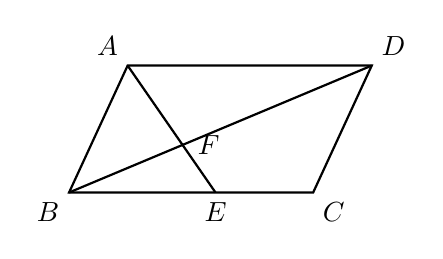
\begin{tikzpicture}[scale=0.62]
\coordinate (B) at (0,0); \coordinate (C) at (5,0); \coordinate (A) at (1.2,2.6); \coordinate (D) at (6.2,2.6);
\coordinate (E) at (3,0); \coordinate (F) at (2.325,0.975);
\draw[thick] (A) -- (B) -- (C) -- (D) -- cycle; \draw[thick] (A) -- (E); \draw[thick] (B) -- (D);
\node[above left] at (A) {$A$}; \node[below left] at (B) {$B$}; \node[below right] at (C) {$C$};
\node[above right] at (D) {$D$}; \node[below] at (E) {$E$}; \node[right=2pt] at (F) {$F$};
\end{tikzpicture}
\end{minipage}
\begin{solution}
$AD \parallel BC$, so $\triangle BFE \sim \triangle DFA$ with $BE : DA = 3 : 5$. Hence $EF : FA = BF : FD = 3 : 5$.\\
Same height: area of $\triangle BFE = \frac35(60) = 36\cm2$ and area of $\triangle DFA = \frac53(60) = 100\cm2$.\\
Area of $\triangle BCD = $ area of $\triangle ABD = 60 + 100 = 160\cm2$.\\
Area of $CDFE = 160 - 36 = 124\cm2$. \quad \textbf{Answer: C} \src{twin of 2018 P2 Q16}
\end{solution}
\end{questions}

\ifdefined\ANSWERS
\begin{center}
\begin{tabular}{*{8}{c}}
\toprule
A1 & A2 & A3 & A4 & A5 & A6 & A7 & A8\\
\midrule
B & C & D & B & D & B & A & C\\
\bottomrule
\end{tabular}
\end{center}
\fi

\newpage
\section*{Section B \quad Paper 1 style (long questions)}

\begin{questions}
\titledquestion{B1}
An inverted right circular conical vessel contains some water. The vessel is held vertically. The depth of water in the vessel is $16\cm{}$. Mary then pours $732\pi\cm3$ of water into the vessel without overflowing. She now finds that the depth of water in the vessel is $20\cm{}$.
\begin{parts}
\part Express the final volume of water in the vessel in terms of $\pi$. \qmarks{3}
\part Mary claims that the final area of the wet curved surface of the vessel is at least $1200\cm2$. Do you agree? Explain your answer. \qmarks{3}
\end{parts}
\begin{solution}
\src{twin of 2016 P1 Q11}
\begin{parts}
\part Let $V\cm3$ be the final volume of water. The water before and after are similar cones.\\
$\dfrac{V - 732\pi}{V} = \left(\dfrac{16}{20}\right)^3$ \mk{1M + 1A}\\
$125V - 125(732\pi) = 64V \implies V = 1500\pi$. The final volume is $1500\pi\cm3$. \mk{1A}
\part Let $r\cm{}$ be the final radius of the water surface. $\frac13\pi r^2(20) = 1500\pi$, so $r = 15$. \mk{1M}\\
Wet curved surface area $= \pi(15)\sqrt{15^2 + 20^2} = 375\pi \approx 1178.1\cm2 < 1200\cm2$ \mk{1M}\\
Thus, the claim is disagreed. \mk{1A f.t.}
\end{parts}
\end{solution}

\titledquestion{B2}
A solid metal sphere of radius $9\cm{}$ is melted and recast into three similar solid right circular cylinders $X$, $Y$ and $Z$. Let $r_1\cm{}$, $r_2\cm{}$ and $r_3\cm{}$ be the base radii of $X$, $Y$ and $Z$ respectively. It is given that $r_1 : r_2 : r_3 = 1 : 2 : 3$.
\begin{parts}
\part Express the volume of $Y$ in terms of $\pi$. \qmarks{3}
\part A craftsman finds that the height of $Y$ is $24\cm{}$.
\begin{subparts}
\subpart Find $r_2$.
\subpart The craftsman claims that the total surface area of $Z$ is greater than the surface area of the sphere. Do you agree? Explain your answer.
\end{subparts}
\hfill(5 marks)
\end{parts}
\begin{solution}
\src{twin of 2026 P1 Q13}
\begin{parts}
\part Volume of the sphere $= \frac43\pi(9^3) = 972\pi\cm3$ \mk{1M}\\
The cylinders are similar, so their volumes are in the ratio $1^3 : 2^3 : 3^3 = 1 : 8 : 27$.\\
Volume of $Y = 972\pi \times \dfrac{8}{1 + 8 + 27} = 216\pi\cm3$ \mk{1M + 1A}
\part
\begin{subparts}
\subpart $\pi r_2^2(24) = 216\pi$ \mk{1M}\\
$r_2^2 = 9$, so $r_2 = 3$. \mk{1A}
\subpart Total surface area of $Y = 2\pi(3^2) + 2\pi(3)(24) = 162\pi\cm2$.\\
$Y$ and $Z$ are similar with $r_2 : r_3 = 2 : 3$, so the total surface area of $Z = 162\pi\left(\frac32\right)^2 = \frac{729}{2}\pi = 364.5\pi\cm2$ \mk{1M}\\
Surface area of the sphere $= 4\pi(9^2) = 324\pi\cm2 < 364.5\pi\cm2$ \mk{1M}\\
Thus, the claim is agreed. \mk{1A f.t.}
\end{subparts}
\end{parts}
\end{solution}

\titledquestion{B3}
The base radius and the curved surface area of a solid metal right circular cone are $7\cm{}$ and $175\pi\cm2$ respectively.
\begin{parts}
\part Find the height of the circular cone. \qmarks{3}
\part The circular cone is divided into a right circular cone $X$ and a frustum $Y$ by a plane which is parallel to its base. The curved surface area of $Y$ is $3$ times the curved surface area of $X$.
\begin{subparts}
\subpart Express the volume of $Y$ in terms of $\pi$.
\subpart If $Y$ is melted and recast into $6$ identical solid spheres, find the diameter of each sphere.
\end{subparts}
\hfill(5 marks)
\end{parts}
\begin{solution}
\src{twin of 2023 P1 Q14}
\begin{parts}
\part Let $\ell\cm{}$ be the slant height. $\pi(7)\ell = 175\pi$, so $\ell = 25$. \mk{1M}\\
Height $= \sqrt{25^2 - 7^2}$ \mk{1M}\\
$\phantom{\text{Height}} = 24\cm{}$ \mk{1A}
\part
\begin{subparts}
\subpart CSA of $X$ : CSA of the whole cone $= 1 : (1 + 3) = 1 : 4$, so their linear ratio is $1 : 2$.\\
Volume of $Y = \frac13\pi(7^2)(24)\left[1 - \left(\dfrac{1}{\sqrt{3 + 1}}\right)^3\right]$ \mk{1M + 1M}\\
$\phantom{\text{Volume of } Y} = 392\pi \times \frac78 = 343\pi\cm3$ \mk{1A}
\subpart Let $d\cm{}$ be the diameter of each sphere.\\
$6 \times \frac43\pi\left(\frac{d}{2}\right)^3 = 343\pi$ \mk{1M}\\
$\left(\frac{d}{2}\right)^3 = \frac{343}{8}$, so $d = 7$. The diameter is $7\cm{}$. \mk{1A}
\end{subparts}
\emph{Trap:} ``3 times'' makes the whole cone $1 + 3 = 4$ times $X$, not 3 times.
\end{parts}
\end{solution}

\titledquestion{B4}
The base of a solid right pyramid is a square of side $30\cm{}$. The height of the pyramid is $20\cm{}$. The pyramid is divided into a frustum $X$ and a pyramid $Y$ by a plane which is parallel to its base. It is given that the height of $Y$ is $12\cm{}$.
\begin{parts}
\part Find the volume of $X$. \qmarks{3}
\part The base of another solid right pyramid is a square. This pyramid is divided into a frustum $Z$ and a pyramid by a plane which is parallel to its base. The height and the total surface area of $Z$ are $4\cm{}$ and $600\cm2$ respectively. Are $X$ and $Z$ similar? Explain your answer. \qmarks{4}
\end{parts}
\begin{solution}
\src{twin of 2024 P1 Q13}
\begin{parts}
\part Volume of $X = \frac13(30^2)(20)\left[1 - \left(\frac{12}{20}\right)^3\right]$ \mk{1M + 1M}\\
$\phantom{\text{Volume of } X} = 6000 \times \frac{98}{125} = 4704\cm3$ \mk{1A}
\part The top of $X$ is a square of side $30 \times \frac{12}{20} = 18\cm{}$. The height of $X$ is $20 - 12 = 8\cm{}$, so the slant height of each face is $\sqrt{\left(\frac{30 - 18}{2}\right)^2 + 8^2} = 10\cm{}$.\\
Area of each lateral face of $X = \frac12(30 + 18)(10) = 240\cm2$ \mk{1M}\\
Total surface area of $X = 4(240) + 30^2 + 18^2 = 2184\cm2$ \mk{1M}\\
$\left(\dfrac{\text{height of } X}{\text{height of } Z}\right)^2 = \left(\dfrac84\right)^2 = 4$ and $\dfrac{\text{TSA of } X}{\text{TSA of } Z} = \dfrac{2184}{600} = 3.64$\\
Since $3.64 \ne 4$, \mk{1M}\\
$X$ and $Z$ are not similar. \mk{1A f.t.}\\
\emph{Trap:} $X$'s height is $8$, not $12$ (that is $Y$'s height).
\end{parts}
\end{solution}

\titledquestion{B5}
A right circular cylindrical container of base radius $9\cm{}$ and height $48\cm{}$ and an inverted right circular conical vessel of base radius $21\cm{}$ and height $42\cm{}$ are held vertically. The container is fully filled with water. The water in the container is now poured into the vessel.
\begin{parts}
\part Find the volume of water in the vessel in terms of $\pi$. \qmarks{2}
\part Find the depth of water in the vessel. \qmarks{4}
\part If a solid metal sphere of radius $12\cm{}$ is then put into the vessel and the sphere is totally immersed in the water, will the water overflow? Explain your answer. \qmarks{3}
\end{parts}
\begin{solution}
\src{twin of 2018 P1 Q14}
\begin{parts}
\part Volume of water $= \pi(9^2)(48)$ \mk{1M}\\
$\phantom{\text{Volume of water}} = 3888\pi\cm3$ \mk{1A}
\part Let $h\cm{}$ be the depth of water. The radius of the water surface is $\frac{21}{42}h = \frac{h}{2}\cm{}$. \mk{1M}\\
$\frac13\pi\left(\frac{h}{2}\right)^2 h = 3888\pi$ \mk{1M + 1A}\\
$h^3 = 46\,656$, so $h = 36$. The depth is $36\cm{}$. \mk{1A}
\part Volume not occupied by water $= \frac13\pi(21^2)(42) - 3888\pi = 6174\pi - 3888\pi = 2286\pi\cm3$ \mk{1M}\\
Volume of the sphere $= \frac43\pi(12^3) = 2304\pi\cm3 > 2286\pi\cm3$ \mk{1M}\\
Thus, the water will overflow. \mk{1A f.t.}
\end{parts}
\end{solution}

\titledquestion{B6}
The height and the base radius of a solid metal right circular cone are $36\cm{}$ and $15\cm{}$ respectively. The circular cone is divided into a circular cone and a frustum $X$ by a plane parallel to its base. It is given that the height of $X$ is $24\cm{}$.
\begin{parts}
\part Express the volume of $X$ in terms of $\pi$. \qmarks{3}
\part Express the total surface area of $X$ in terms of $\pi$. \qmarks{3}
\part $X$ is melted and recast into a solid cube. Does the total surface area of the cube exceed the total surface area of $X$? Explain your answer. \qmarks{3}
\end{parts}
\begin{solution}
\src{twin of 2025 P1 Q14}
\begin{parts}
\part The small cone removed has height $36 - 24 = 12\cm{}$ and base radius $15 \times \frac{12}{36} = 5\cm{}$. \mk{1M}\\
Volume of $X = \frac13\pi(15^2)(36) - \frac13\pi(5^2)(12)$ \mk{1M}\\
$\phantom{\text{Volume of } X} = 2700\pi - 100\pi = 2600\pi\cm3$ \mk{1A}
\part Slant heights: $\sqrt{15^2 + 36^2} = 39\cm{}$ and $\sqrt{5^2 + 12^2} = 13\cm{}$. \mk{1M}\\
TSA of $X = \left[\pi(15)(39) - \pi(5)(13)\right] + \pi(15^2) + \pi(5^2)$ \mk{1M}\\
$\phantom{\text{TSA of } X} = 520\pi + 225\pi + 25\pi = 770\pi\cm2$ \mk{1A}
\part Let $s\cm{}$ be the side of the cube. $s^3 = 2600\pi$, so $s = \sqrt[3]{2600\pi} \approx 20.139$. \mk{1M}\\
TSA of the cube $= 6s^2 \approx 2433.5\cm2$ \mk{1M}\\
TSA of $X = 770\pi \approx 2419.0\cm2 < 2433.5\cm2$\\
Thus, the total surface area of the cube exceeds the total surface area of $X$. \mk{1A f.t.}\\
\emph{Trap:} the frustum has \emph{two} circular faces, $225\pi$ and $25\pi$; both belong in the total.
\end{parts}
\end{solution}
\end{questions}

\ifdefined\ANSWERS\else
\vfill
{\color{wyred}\rule{\linewidth}{0.8pt}}\par
\small\textbf{Self-check:} \
$\square$ $\pi$ kept to the last line \
$\square$ both numbers, the comparison and a conclusion \
$\square$ $k$ measured from the vertex \
$\square$ square root of an area ratio before cubing
\fi

\end{document}
